\chapter{Background}

\section{The \Beluga Language}

In \Beluga, theorems are encoded using contextual \LF, its index language, and proofs are encoded as programs.
Logic propositions are represented as \LF type families with term-level constants parameterized by $\beta$-normal $\eta$-long \LF terms to construct witnesses for these propositions~\cite{nanevski2008contextual, foundation2008pientka, DBLP:journals/corr/abs-1009-2789}.
To facilitate the implementation of semantic analysis, and because \LF kinds, types and terms are strongly normalizing~\cite{harper1993framework}, they are required to be encoded in normal form by the user.
\Beluga extends \LF to support explicit contexts and substitutions, which enables mechanized reasoning with respect to assumptions, like in proofs on paper~\cite{pientka2010programming}.
This means that terms containing free variables can be manipulated and reasoned about explicitly in \Beluga.

To illustrate how \Beluga is leveraged to mechanically prove properties about formal systems, consider the following example adapted from \cite{felty2010reasoning} where it is shown that algorithmic equality for an untyped $\lambda$-calculus is reflexive.
The abstract syntax for this calculus is first defined in figure~\ref{figure:running-example-abstract-syntax}, which is encoded as an \LF type constant \verb|term| with term constants \verb|lam|, \verb|app| and \verb|unit| in the \verb|Term| module of figure~\ref{figure:running-example-implementation}.
Then, the algorithmic equality judgment for terms is defined in figure~\ref{figure:running-example-equality} and encoded as an \LF type family \verb|≡|, using an infix notation, in module \verb|Algorithmic_equality|.
Note that this definition for equality does not provide constants to construct witnesses of reflexivity, symmetry nor transitivity.
These properties may instead be derived, like theorem~\ref{theorem:reflexivity} proving that reflexivity holds.
This corresponds to the \verb|refl| recursive program of figure~\ref{figure:running-example-implementation} which constructively shows that for any (possibly open) term $M$, the algorithmic equality $M \equiv M$ holds.
The notion that $M$ may contain free variables comes into play when proving reflexivity for terms of the form $\lambda x. M$ since the induction hypothesis requires assumptions about the function parameter $x$.

\begin{figure}[H]
\begin{subfigure}{\linewidth}
\centering
\begin{tabular}{p{2cm} >{\raggedleft}p{1cm} r l}
Terms & $M, N$ & $\Coloneqq$ & $x \mid \lambda x. M \mid M\ N \mid \Unit$
\end{tabular}
\caption{%
Syntax definition for the untyped $\lambda$-calculus used in the running example.
}
\label{figure:running-example-abstract-syntax}
\end{subfigure}
\par\bigskip
\begin{subfigure}{\linewidth}
\begin{mdframed}[frametitle={$\boxed{\Gamma \vdash M \equiv N}$ : the term $M$ is algorithmically equal to $N$ in context $\Gamma$}]
\begin{equation}
\infer[\equiv\text{-lam}]{\Gamma \vdash \lambda x. M \equiv \lambda x. N}{\Gamma, x : \mathsf{term}, e : x \equiv x \vdash M\ x \equiv N\ x}
\end{equation}
\begin{equation}
\infer[\equiv\text{-app}]{\Gamma \vdash M_1\ M_2 \equiv N_1\ N_2}{\Gamma \vdash M_1 \equiv N_1 & \Gamma \vdash M_2 \equiv N_2}
\end{equation}
\begin{equation}
\infer[\equiv\text{-unit}]{\Gamma \vdash \Unit \equiv \Unit}{}
\end{equation}
\end{mdframed}
\caption{Definition of algorithmic equality over the untyped terms.}
\end{subfigure}
\caption[Running example of algorithmic equality for an untyped $\lambda$-calculus]{%
Running example.
}
\label{figure:running-example-equality}
\end{figure}%
\begin{figure}\ContinuedFloat
\begin{subfigure}{\linewidth}
\begin{theorem}
\label{theorem:reflexivity}
If $\Gamma$ is a context where $(x : \mathsf{term}) \in \Gamma$ is sufficient for $(e : x \equiv x) \in \Gamma$, and $\deduce{\Gamma \vdash \Term{M}}{\D}$, then $\Gamma \vdash M \equiv M$.
\end{theorem}
{\footnotesize
\begin{proof}
By structural induction on $\D$:
\begin{itemize}
\item
Case $\D = \infer[\text{term-var}]{\Gamma \vdash \Term{x}}{\deduce{(x : \mathsf{term}) \in \Gamma}{\D'}}$.
\par
By the regular context specification on $ \D' $, we have $(e : x \equiv x) \in \Gamma$, hence $\Gamma \vdash x \equiv x$.
\item
Case $\D = \infer[\text{term-lam}]{\Gamma \vdash \Term{\lambda x. N}}{\deduce{\Gamma, x : \mathsf{term} \vdash \Term{N}}{\D'}}$.
\par
By weakening on $\D'$, we have $\deduce{\Gamma, x : \mathsf{term}, e : x \equiv x \vdash \Term{N}}{\E}$.
\par
By the induction hypothesis on $\E$, we have $\deduce{\Gamma, x : \mathsf{term}, e : x \equiv x \vdash N\ x \equiv N\ x}{\E'}$.
\par
Then,
\begin{equation*}
\infer[\equiv\text{-lam}]{\Gamma \vdash \lambda x. N \equiv \lambda x. N}{\deduce{\Gamma, x : \mathsf{term}, e : x \equiv x \vdash N\ x \equiv N\ x}{\E'}}.
\end{equation*}
\item
Case $\D = \infer[\text{term-app}]{\Gamma \vdash \Term{M_1\ M_2}}{\deduce{\Gamma \vdash \Term{M_1}}{\D_1} & \deduce{\Gamma \vdash \Term{M_2}}{\D_2}}$.
\par
By the induction hypothesis on $\D_1$, we have $\deduce{\Gamma \vdash M_1 \equiv M_1}{\E_1}$.
\par
By the induction hypothesis on $\D_2$, we have $\deduce{\Gamma \vdash M_2 \equiv M_2}{\E_2}$.
\par
Then,
\begin{equation*}
\infer[\equiv\text{-app}]{\Gamma \vdash M_1\ M_2 \equiv M_1\ M_2}{\deduce{\Gamma \vdash M_1 \equiv M_1}{\E_1} & \deduce{\Gamma \vdash M_2 \equiv M_2}{\E_2}}.
\end{equation*}
\item
Case $\D = \infer[\text{term-unit}]{\Gamma \vdash \Term{\Unit}}{}$.
\par
This case holds by $\equiv\text{-unit}$.
\end{itemize}
\end{proof}
}
\caption{On paper proof of algorithmic equality for this $\lambda$-calculus.}
\end{subfigure}
\caption[]{Running example (contd.).}
\end{figure}%
\begin{figure}\ContinuedFloat
\begin{subfigure}{\linewidth}
\begin{Verbatim}[commandchars=\\\{\}, baselinestretch=1, numbers=left]
\verbbf{module} Term = \verbbf{struct}
  \verbbf{LF} term : \verbbf{type} =
  | lam : (term \makebox[1em]{→} term) \makebox[1em]{→} term
  | app : term \makebox[1em]{→} term \makebox[1em]{→} term
  | unit : term;
  \verbprag{--name term M.}
\verbbf{end}
\verbbf{module} Algorithmic_equality = \verbbf{struct}
  \verbprag{--open Term.}
  \verbprag{--infix \makebox[1em]{≡} none.}
  \verbbf{LF} \makebox[1em]{≡} : term \makebox[1em]{→} term \makebox[1em]{→} \verbbf{type} =
  | lam : (\{x : term\} \makebox[1em]{→} x \makebox[1em]{≡} x \makebox[1em]{→} M x \makebox[1em]{≡} N x) \makebox[1em]{→} Term.lam M \makebox[1em]{≡} Term.lam N
  | app : M1 \makebox[1em]{≡} N1 \makebox[1em]{→} M2 \makebox[1em]{≡} N2 \makebox[1em]{→} Term.app M1 M2 \makebox[1em]{≡} Term.app N1 N2
  | unit : Term.unit \makebox[1em]{≡} Term.unit;
\verbbf{end}
\verbprag{--open Term.}
\verbprag{--open Algorithmic_equality.}
\verbbf{schema} ctx = \verbbf{block} (x : term, eq : x \makebox[1em]{≡} x);
\verbbf{rec} refl : (g : ctx) \makebox[1em]{→} \{M : [g \makebox[1em]{⊢} term]\} \makebox[1em]{→} [g \makebox[1em]{⊢} M \makebox[1em]{≡} M] =
  / total d (refl _ d) /
  \verbbf{mlam} M \makebox[1em]{⇒}
    \verbbf{case} [_ \makebox[1em]{⊢} M] \verbbf{of}
    | [g \makebox[1em]{⊢} #p.x] \makebox[1em]{⇒} [g \makebox[1em]{⊢} #p.eq]
    | [g \makebox[1em]{⊢} Term.lam {\textbackslash}x. F] \makebox[1em]{⇒}
        \verbbf{let} [g, b : \verbbf{block} (x : term, eq : x \makebox[1em]{≡} x) \makebox[1em]{⊢} D] =
          refl [g, b : \verbbf{block} (x : term, eq : x \makebox[1em]{≡} x) \makebox[1em]{⊢} F[\monoellipsis, b.x]]
        \verbbf{in}
        [g \makebox[1em]{⊢} Algorithmic_equality.lam {\textbackslash}x. {\textbackslash}eq. D[\monoellipsis, <x; eq>]]
    | [g \makebox[1em]{⊢} Term.app M1 M2] \makebox[1em]{⇒}
        \verbbf{let} [g \makebox[1em]{⊢} D1] = refl [g \makebox[1em]{⊢} M1] \verbbf{in}
        \verbbf{let} [g \makebox[1em]{⊢} D2] = refl [g \makebox[1em]{⊢} M2] \verbbf{in}
        [g \makebox[1em]{⊢} Algorithmic_equality.app D1 D2]
    | [g \makebox[1em]{⊢} Term.unit] \makebox[1em]{⇒} [g \makebox[1em]{⊢} Algorithmic_equality.unit];
\end{Verbatim}
\caption[Algorithmic equality in \Beluga]{%
Mechanized proof of algorithmic equality in \Beluga for this $\lambda$-calculus, adapted from \cite{felty2010reasoning}.
}
\label{figure:running-example-implementation}
\end{subfigure}
\caption[]{Running example (contd.).}
\label{figure:running-example}
\end{figure}

\clearpage

As illustrated in figure~\ref{figure:running-example-implementation}, a signature in \Beluga is the list of all the toplevel constant declarations in a mechanization.
This includes the aforementioned \LF type-level and term-level constant declarations, but also includes inductive and coinductive type declarations at the computation-level, with their associated constructors and destructors respectively, and computation-level programs.
\Harpoon provides an alternative to specifying proofs as programs in the form of a proof script comprised of tactics and their effects on the meta-level and computation-level contexts for variables.
A complete specification of the concrete syntax for signature-level declarations is provided in section~\ref{section:syntax-signature} as part of grammars for parsing.
To discuss the statics and dynamics of \Beluga, an abstract syntax definition like the following is used instead.

Let $x$ and $c$ range over computation-level variables and constants respectively, $X$ range over meta-object variables, $\psi$ over context variables and $g$ over context schemas.
Figure~\ref{figure:internal-syntax} then provides an overview of \Beluga's core language.
\LF kinds classify \LF types, which classify \LF terms.
Likewise, computation-level kinds classify computation-level types, which classify computation-level expressions.
\LF terms are broken down into normal and neutral terms, along with heads and spines, to syntactically enforce canonical forms.
The notation $A \to K$ is used for the \LF kind $\Pi x{:}A. K$ when $x$ does not appear free in $K$.
The notation $A \to B$ is defined analogously for \LF types.
Since \Beluga's type system is bidirectional, the syntax of computation-level expressions is split into those for which a type can be inferred (type-synthesizing expressions), and those that can be checked against a type (type-checkable expressions).
Meta-objects, classified by meta-types, can be embedded in the computation-level by way of boxes that simultaneously bind all variables from \LF contexts.

\begin{figure}
\begin{subfigure}{\linewidth}
\begin{tabular}{p{5.5cm} >{\raggedleft}p{1cm} r l}
\LF kinds & $K$ & $\Coloneqq$ & $\Pi x{:}A. K \mid \mathbf{type}$\\
\LF types & $A, B$ & $\Coloneqq$ & $\Pi x{:}A. B \mid P$\\
Atomic \LF types & $P$ & $\Coloneqq$ & $a \cdot S$\\
\LF normal terms & $M$ & $\Coloneqq$ & $R \mid \lambda x. M$\\
\LF neutral terms & $R$ & $\Coloneqq$ & $H \cdot S \mid u[\sigma]$\\
\LF heads & $H$ & $\Coloneqq$ & $x \mid c \mid p[\sigma]$\\
\LF spines & $S$ & $\Coloneqq$ & $\cdot \mid M\ S$\\
Substitutions & $\sigma$ & $\Coloneqq$ & $\cdot \mid \mathsf{id}_\psi \mid \sigma, M \mid \mathsf{id}_\psi[\rho]$\\
Substitution closures & $\rho$ & $\Coloneqq$ & $s[\sigma]$\\
Contexts & $\Psi$ & $\Coloneqq$ & $\cdot \mid \psi \mid \Psi, x : A$\\
\end{tabular}
\caption{Internal syntax of contextual \LF in \Beluga.}
\end{subfigure}
\par\bigskip
\begin{subfigure}{\linewidth}
\begin{tabular}{p{5.5cm} >{\raggedleft}p{1cm} r l}
Meta-types & $U$ & $\Coloneqq$ & $\cdots \mid g \mid (\Psi \vdash A) \mid (\Psi \vdash \Psi)$\\
Meta-objects & $C$ & $\Coloneqq$ & $\cdots \mid \Psi \mid (\Psi \vdash M) \mid (\Psi \vdash \sigma)$
\end{tabular}
\caption{Internal syntax of \Beluga's meta level (excerpt).}
\end{subfigure}
\par\bigskip
\begin{subfigure}{\linewidth}
\begin{tabular}{p{5.5cm} >{\raggedleft}p{1cm} r l}
Computation-level kinds & $\kappa$ & $\Coloneqq$ & $[U] \to \kappa \mid \Pi X{:}U. \kappa \mid \mathbf{ctype}$\\
Computation-level types & $\tau$ & $\Coloneqq$ & $\cdots \mid c \mid \tau_1 \to \tau_2 \mid \Pi X{:}U. \tau \mid [U] \mid \tau\ [C]$\\
Type-checkable expressions & $e$ & $\Coloneqq$ & $\cdots \mid i \mid [C] \mid \mathbf{fn}\ x \Rightarrow e \mid \mathbf{mlam}\ X \Rightarrow e$ \\
& & $|$ & $\mathbf{let}\ x = i\ \mathbf{in}\ e \mid \mathbf{case}\ i\ \mathbf{of}\ \overrightarrow{p \Rightarrow e}$\\
Type-synthesizing expressions & $i$ & $\Coloneqq$ & $\cdots \mid x \mid c \mid i \ e \mid e : \tau$
\end{tabular}
\caption{Internal syntax of \Beluga's computation level (excerpt).}
\end{subfigure}
\caption[Excerpt of \Beluga's internal syntax]{%
Excerpt of \Beluga's internal syntax~\cite{nanevski2008contextual, germain2010implementation, cave2013first, ferreira2013compiling} used in discussions about its theory.
}
\label{figure:internal-syntax}
\end{figure}

\section{The Legacy Implementation of \Beluga} \label{section:beluga-implementation}

This section presents an overview of the implementation of \Beluga before any contribution detailed in this thesis were made\footnote{The implementation of \Beluga at revision hash \href{https://github.com/Beluga-lang/Beluga/tree/3db1ffd08d4c3bde7ad2ceb924bfb95488eef2b2}{3db1ffd08d4c3bde7ad2ceb924bfb95488eef2b2, available on GitHub.}}.
This initial description serves as the basis for all performance and design comparisons made with respect to \Beluga version~\texttt{1.1}.

\Beluga is implemented following the pipeline architectural pattern, whereby processing of a signature is implemented in distinct phases, and data flows in a feed-forward fashion throughout.
The compilation of \Beluga programs to machine code is not supported, so the implementation only covers the frontend component of compilation, which is responsible for syntactic and semantic analysis of programs.
Since \Beluga is a dependently-typed language featuring code coverage analysis and termination checking, this semantic analysis process is complex.

\begin{figure}
\centering
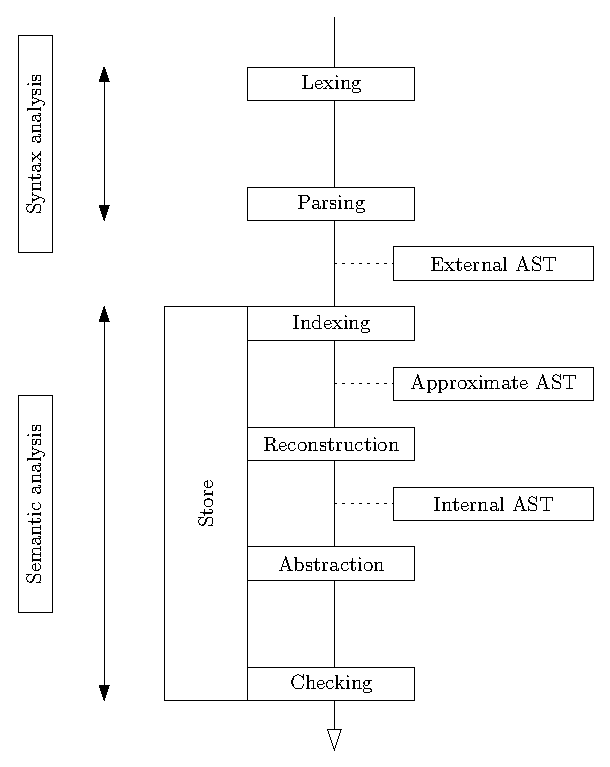
\includegraphics{figures/legacy-beluga-processing-pipeline.eps}
\caption[Overview of \Beluga version \texttt{1.0}'s processing pipeline]{%
Overview of the implementation of \Beluga version \texttt{1.0}'s processing pipeline.
The syntax analysis process converts the textual representation of \Beluga programs into an initial \acs{AST}.
The semantic analysis process refines this \acs{AST} by performing type-directed signature reconstruction, using global mutable data structures that include a store of constant declarations in the signature.
}
\label{figure:legacy-beluga-processing-pipeline}
\end{figure}

As illustrated in figure~\ref{figure:legacy-beluga-processing-pipeline}, the processing of a \Beluga signature starts with syntax analysis, which is comprised of a tokenization and parsing phase that converts the textual representation of the signature to an \ac{AST}, called the external \ac{AST}.
The model for this \ac{AST} contains ambiguous nodes, meaning that some \ac{AST} node variants capture multiple parse trees.
Specifically, the application of \LF type-level and term-level constants is represented as a list of parsemes, which effectively postpones the parsing of applications featuring user-defined operator notations.
Parsing of signature-level declarations also features auxiliary data and routines for mixing or unmixing parsemes to delegate some disambiguation to phases after context-free parsing.

Indexing in \Beluga is the process by which the concrete syntax is elaborated to a locally nameless representation called the approximate syntax, wherein bound variables are replaced with their corresponding de Bruijn indices, and constant names are replaced with symbolic identifiers defined in the centralized store of declarations.
For instance, the \LF term $\lambda x. \lambda y. \lambda z.\ x\ z\ (y\ z)$ is indexed as $\lambda\ \lambda\ \lambda\ 3\ 1\ (2\ 1)$.
As part of \Beluga's design for terse type declarations and programs, the computation of de Bruijn indices for some free variables is postponed until the abstraction phase.
Indexing is run after parsing, and is additionally responsible for disambiguating the juxtaposition of \LF parsemes at the precedence level of applications (which may contain user-defined operators), as well as disambiguating \LF types from terms and resolving constants.
This design is sensible since computing de Bruijn indices requires a stateful traversal of the \ac{AST} that accumulates lists of bindings to produce the referencing environment.
Using the store, some measure of identifier overloading is supported using a pre-defined order of lookups in the referencing environment based on the kind of identifier that is expected for a given \ac{AST} node.
For instance, computation-level identifiers are resolved by looking up in order the store of computation-level variables, the store of program constants, and then the store of data type constructors.
Since names appearing in the \LF level are not part of this name resolution strategy, then an identifier can be overloaded to stand for an \LF term as well as a computation-level expression.

After indexing, the reconstruction~\cite{pientka2013insider} phase is run to reconstruct holes in types and terms, both at the \LF level and the computation level.
These holes stand for arguments omitted by the user, and provide an elegant way of abbreviating otherwise tedious aspects of programming with dependent types.
For instance, in the \verb|refl| program of figure~\ref{figure:running-example-implementation}, the context parameter \verb|(g : ctx)| is implicit, meaning that calls like \verb|refl m| actually denote \verb|refl _ m|, with a hole \verb|_| where a context argument is expected.
This is admissible because any argument for that parameter can be reconstructed from \verb|m| given for the explicit parameter \verb|{M : [g ⊢ term]}|, which is defined with respect to \verb|g|.
At the \LF level, approximate types are constructed to partially check the kinding of \LF types and the typing of \LF terms, as well as for guiding the synthesis of normal terms that check against a given type using typing constraints.
Type-driven unmixing of overloaded syntactic forms occurs at the meta-level, whereby meta-objects are disambiguated from substitutions during reconstruction.
The approximate \ac{AST} provides a disambiguated representation of the overall \Beluga signatures, which helps in keeping track of the various changes made during this complicated phase.

A nearly complete internal \ac{AST} as defined in figure~\ref{figure:internal-syntax} is produced at the end of reconstruction.
An abstraction phase~\cite{germain2010implementation} is run to abstract over free variables, which effectively introduces binders for implicit parameters, and unrolls the contexts of variables used during type-driven reconstruction.
For instance, the \LF term constant \verb|Algorithmic_equality.app| of figure~\ref{figure:running-example-implementation} is abstracted to

\bigskip
\begin{Verbatim}[commandchars=\\\{\}, baselinestretch=1]
(M1 : term) → (N1 : term) → (M2 : term) → (N2 : term) →
  (_ : M1 \makebox[1em]{≡} N1) \makebox[1em]{→} (_ : M2 \makebox[1em]{≡} N2) \makebox[1em]{→} Term.app M1 M2 \makebox[1em]{≡} Term.app N1 N2
\end{Verbatim}

\noindent
and then de Bruijn indices are recomputed, which yields
\begin{equation*}
\Pi_{\texttt{term}}\ \Pi_{\texttt{term}}\ \Pi_{\texttt{term}}\ \Pi_{\texttt{term}}\ \Pi_{4 \equiv 3} \Pi_{3 \makebox[1em]{≡} 2}\ \texttt{Term.app}\ 6\ 4\ \equiv \texttt{Term.app}\ 5\ 3
\end{equation*}
This phase completes the desugaring of \Beluga programs since it finishes the computation of de Bruijn indices for variables across all levels.
The main technical challenge abstraction runs into is determining the order in which introduced binders must appear so that dependencies on terms are preserved in inferred dependent types.
This includes identifying and handling circular dependencies in abstracted parameters.

Finally, a semantic checking phase is run to ensure signature reconstruction and abstraction yielded valid programs.
This includes performing type-checking, coverage-checking and totality-checking.
These processes guarantee, respectively, that \LF-level and computation-level expressions are well-typed, that case analyses are exhaustive, and that functions annotated with a totality declaration terminate for all inputs.
Typing and coverage constraints generated during theses checking processes are statefully shared throughout this phase.
Leftover and unresolved constraints in the state after having fully processed a program unit are used to signal to the user that that program is unsound within \Beluga's system.

The flow of data in the implementation of \Beluga is complex, like in most software systems.
Starting with the indexing phase, data is shared between the phases of signature reconstruction using a global mutable store.
This auxiliary data structure is a set of tables mapping constant identifiers to metadata, like in a relational database.
Crucially, the referencing environment used during indexing is computed using this store.
At any given point during the processing pipeline, the store's state is valid since program units are processed sequentially.
New program units may be safely appended afterwards in interactive sessions.

The \Beluga system provides two ways to interactively perform queries on an existing \Beluga signature, or to augment it with new theorems.
These are the legacy \ac{REPL} and the \Harpoon system~\cite{errington2021harpoon}, the latter of which is designed as a replacement for the former.
Both systems allow the user to input \LF-level terms or computation-level expressions and get their type inferred with respect to an already elaborated \Beluga signature.
\Harpoon further enables the interactive definition and proving of theorems using sets of tactics aimed at automating proof development.
Both the \ac{REPL} and \Harpoon depend on the earlier processing phases of \Beluga and the flow of information therein.

This thesis focuses on the first few phases of the \Beluga processing pipeline, specifically parsing and indexing.
Rearchitected solutions to those phases are then shown to provide better support for some of \Beluga's and \Harpoon's existing features, while also addressing usability and soundness issues.

\section{State Management and Incremental Program Development}\label{section:intro-state-management}

Users benefit from interacting with the code they are editing by way of auxiliary software that performs actions on it.
Incremental program development in programming language tooling is the problem of applying edit actions to programs while only reprocessing a minimal portion of the program under edit.
The kinds of edit actions that can be implemented vary from one programming language to the other depending on the language's features.
Typically, edit actions include software refactoring commands such as variable renaming, reordering functions in a file, selecting a list of statements from one function and extracting them into a separate function, pretty-printing and formatting the textual representation of code, etc.
Sound and efficient handling of these edit actions is instrumental to the productivity of users working on large scale software systems.
This problem of incremental program development arises in \Beluga and \Harpoon because of the interactive tooling they provide for editing proofs, which are represented as programs.

% What is the key problem in incremental program development?

Throughout syntactic and semantic analyses pipelines, data is accumulated during the processing of any given program unit.
This data raises one of the more challenging aspects in implementing incremental program development, and the main motivation for reworking \Beluga's processing pipeline: \textit{a program unit may only be revisited with the processing state it was defined in}.
This means, for instance, that a procedure performing name lookups or mutations on an \ac{AST} at a given node may only do so using the variables and declarations in scope at that \ac{AST} node, just as the user does when editing the textual representation of that \ac{AST} node.
As such, edit actions on an \ac{AST} must preserve its semantic correctness properties so that serializing and subsequently deserializing it produces the same \ac{AST} and processing state.

% What is the preliminary step to supporting incremental program development?

A preliminary step to supporting incremental program development is to parameterize the processing routines with respect to a visitor state.
As such, those routines can be used in an out-of-order fashion as opposed to when the program is processed during compilation tasks.
This is because the routine can be visited with a different state than the one that is naturally constructed when sequentially processing program units.
For instance, a routine like conflict-avoiding variable renaming can be dependent on a referencing environment to perform variable and constant lookups.
If such a routine is invoked during an interactive program development session, then a separate routine can be implemented to rebuild the referencing environment without having to reprocess the entire program and its dependencies.
In this case, the edit action requires visiting a selected \ac{AST} node with the referencing environment as visitor state.
The issue then becomes how to efficiently construct and preserve the correctness of such visitor states.
As it pertains to \Beluga and \Harpoon, this specifically affects \ac{REPL} sessions instantiated at program holes.
